\rhead{Шемякин}
\subsection{Законы Де Моргана}
	
	\begin{theorem*}
		\begin{equation}
			Y \setminus\left(\bigcup\limits_{\alpha \in A} X_\alpha \right) = \bigcap\limits_{\alpha \in A} \left( Y \setminus X_\alpha \right) 
		\end{equation}
		
		\begin{equation}
			Y \setminus\left(\bigcap\limits_{\alpha \in A} X_\alpha \right) = \bigcup\limits_{\alpha \in A} \left( Y \setminus X_\alpha \right) 
		\end{equation}
		
		\begin{equation}
			Y \bigcap \left(\bigcup\limits_{\alpha \in A} X_\alpha \right) =  \bigcup\limits_{\alpha \in A} \left(Y \bigcap X_\alpha \right)
		\end{equation}
		
		\begin{equation}
			 Y \bigcup \left(\bigcap\limits_{\alpha \in A} X_\alpha \right) =  \bigcap\limits_{\alpha \in A} \left(Y \bigcup X_\alpha \right)
		\end{equation}
	\end{theorem*}
	
	\begin{proof}
		 Докажем (1), остальные аналогично (см. фото)
		 $$ x \in \text{левой части} \Leftrightarrow (x \in Y) \text{ и } \left(x \notin \bigcup\limits_{\alpha \in A} X_\alpha \right) \Leftrightarrow x \in Y \text{ и } \forall \alpha \in A \ \ x \notin X_\alpha \Leftrightarrow $$  $$ \Leftrightarrow \forall \alpha \in A ~ \left(x \notin X_\alpha \text{ и } x \in Y \right) \\ \Leftrightarrow  \forall \alpha \in A \ \ x \in (Y \setminus X_\alpha) \Leftrightarrow \bigcap\limits_{\alpha \in A} \left (Y \setminus X_\alpha \right) $$
	\end{proof}
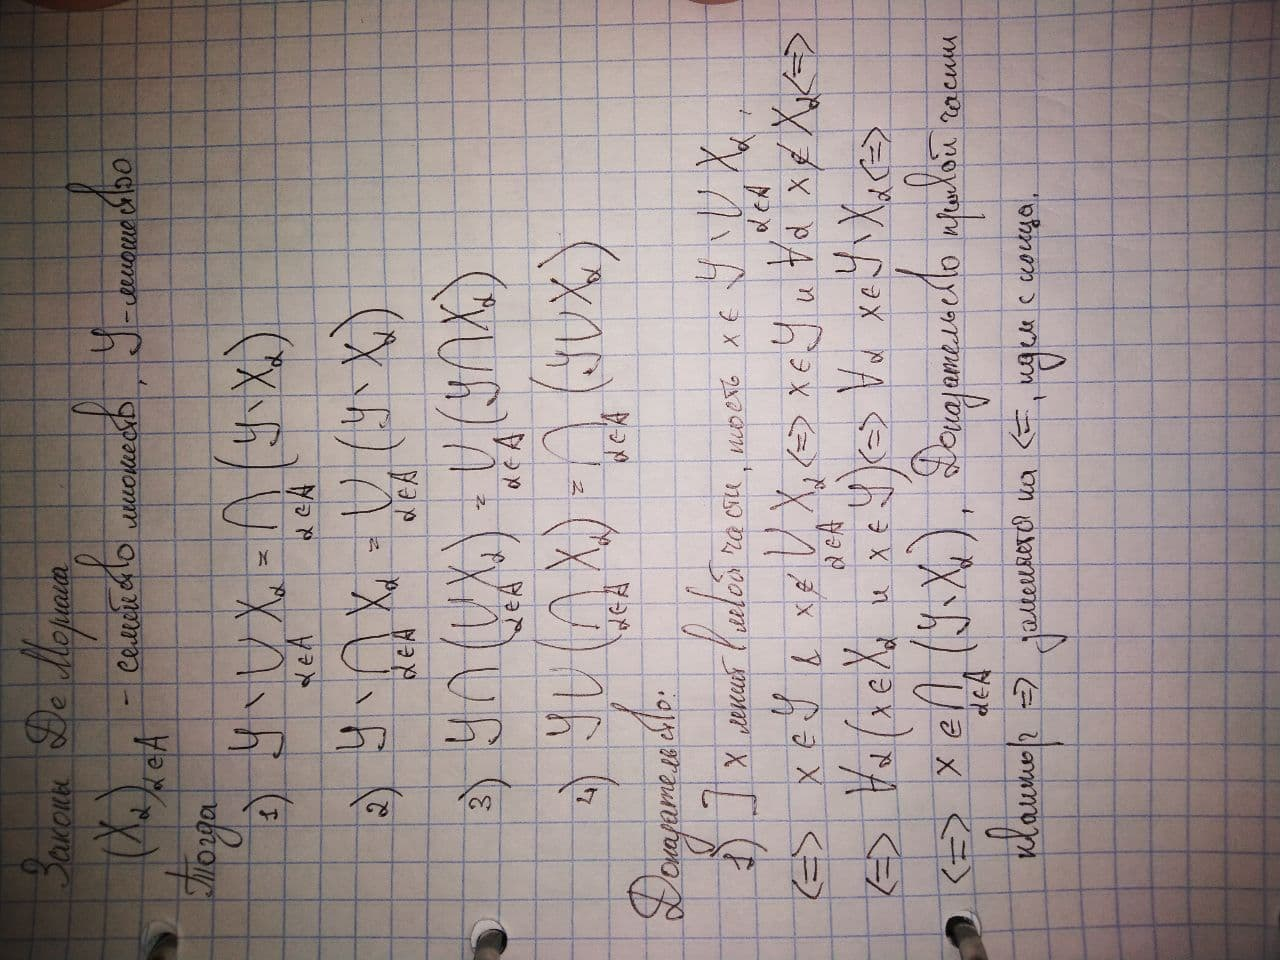
\includegraphics[height = 0.7\textheight, width = \textwidth]{Images/законы деморгона.jpg}
% Вроде норм получилось

% к сожалению в латексе нет значков для записи объедение по альфа
% к счастью есть :)
% $\bigcup\limits_{\alpha \in A} G_\alpha$

% поэтому вот вам картинки, слов тут все равно не много
%как кстати нормально картинки встасить

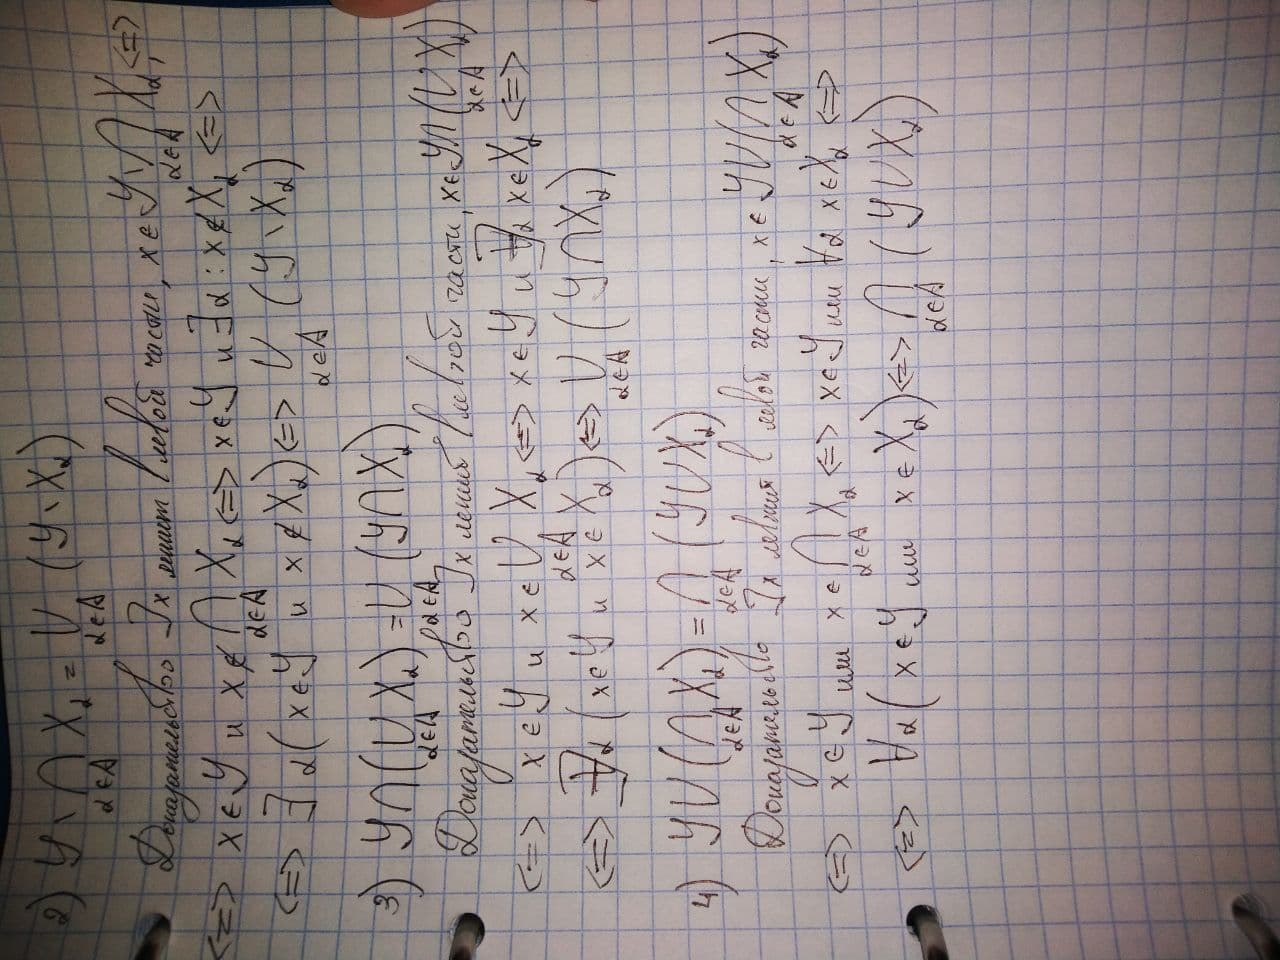
\includegraphics[width =\textwidth, height = 0.8\textheight]{Images/доказательства де моргана.jpg}
% Вроде норм получилось

%техать мы это не будем по причине кванторы

% ленивая жопа

\newpage
\subsection{Единственность предела и ограниченность сходящейся последовательности}
\begin{definition}
     Последовательность $ { ( {x_{n}} )_{n \varepsilon  {N} }}$ - семейство, заиндексированное натуральными числами.
\end{definition}

    %  ${x_{n}}\varepsilon  R$ 
     
    %  Пусть есть $ { ( {x_{n}} )_{n \varepsilon  {N} }}$ и $a \varepsilon  R$
     
    % $ {x_{n}} \rightarrow a$ 
    
    % $\lim\limits_{n \to \infty} x_n = a$
    
    % %как в формулы пробела вставить а       
    
    % $\forall \varepsilon > 0 \ \exists N \  \forall n > N: \abs{{x_{n}} - a} < \varepsilon$ \\
    
    % (Расстояние от ${x_{n}}$ до $a$) $< \varepsilon \Leftrightarrow \abs{{x_{n}} - a} < \varepsilon$ 
    
    % Примеры:
    % \begin{enumerate}
    %     \item ${x_{n}}$ - стационарная последовательность $x_n = a$ 
        
    %     $\lim\limits_{n \to \infty} x_n = a$
        
    %     \item $x_n = \frac{1}{n}$ тогда $x_n \longrightarrow 0$
        
    %     $\forall \ \varepsilon > 0 \  \exists N = \frac{1}{\varepsilon} \ \forall \  n > \frac{1}{\varepsilon} \ \ \frac{1}{n} < \varepsilon$
        
    %     \item $x_n = (-1)^{n}$ Расходится
        
    %     $\forall \ \varepsilon > 0 \  \exists N  \ \forall \  n > N \ \ \abs{x_n - a} < \varepsilon$
        
    %     заменим $N$ на $N(\varepsilon)$ N от епсилон. Тогда $ \forall n > N(\varepsilon) \  \abs{x_n - a} < \varepsilon$
        
    %     Тоесть $(N(\varepsilon); \infty)$
        
    %     Тогда рассмотрим для конкретного $\varepsilon = 1 \ \exists N(1) \ \forall \ n > N(1) \ \ \abs{x_n - a} < 1$
        
    % \end{enumerate}
    % \quad
    \begin{theorem*} (О единственности предела)
        $x_n$- последовательность в метрическом пространстве $(X, \rho)$
        
        $a, b \in X$, $x_n \to a$, $x_n \to b \Rightarrow a = b$
    \end{theorem*}
    
    \begin{proof}
        Предположим $a \neq b$, следовательно существуют окрестности точек $a$ и $b$, что они не пересекаются: 
        
        $U(a) = B_1(a, \frac{1}{2}r) \ \ \ \ V(b) = B_2(b, \frac{1}{2}r)$ 
        
        $r = \rho(a,b)$
        
        Докажем от противного, что эти шары  $B_1$  и $B_2$ не пересекаются.
        
        Пусть $z \in B_1$ и $z \in B_2$ - точка пересечения
        
        $\rho(a, z) < \frac{1}{2} r$
        
        $\rho(b, z) < \frac{1}{2} r$
        
        $\rho(a, b) = r > \rho(a, z) + \rho(z, b)  \Rightarrow \frac{1}{2}r + \frac{1}{2}r < r$ {---} противоречие по неравенству треугольников $\Rightarrow$ шары не пересекаются
         
        Рассмотрим непересекающиеся окрестности $U(a), V(b)$. Вне $U(a)$ конечное число членов последовательности $\Longrightarrow$ в $V(b)$ конечное число членов последовательности. Получили противоречие.
    \end{proof}
    
    \begin{theorem*} (Об ограничености сходящейся последовательности)
        В метрическом пространстве сходящаяся последовательность ограниченна.
        
        Последовательность $x_n$ ограниченна, если множество ее значений ограниченно.
    \end{theorem*}
    \begin{proof}
        Для $\varepsilon = 1 \ \ \exists N \ \forall n > N \ \ q(x_n, a) < 1$ определение предела для $\varepsilon = 1$
        
        $R = max(q(x_i, a))$ Берем конечные точки и раширяем шар до максимального среди них радиуса. Откуда $x_n \subset B(a, R)$.
    \end{proof}
    
\newpage
\subsection{Теорема о предельном переходе в неравенствах для последовательностей и для функций}
    \begin{theorem*}
    $x_n , y_n$ - вещественные последовательности.
    
    $a, b \in X$, $x_n \to a$, $x_n \to b$. Если $\forall n \in N \ \ x_n \leqslant y_n \Rightarrow a \leqslant b$.
    \end{theorem*}
    \begin{proof}
    Докажем от противного.
    
    Пусть $b < a$
    
    $\varepsilon = \frac{a - b}{2}$ растояние от $a$ до $b \Rightarrow b + \varepsilon = a - \varepsilon$
    
    Для этого же $\varepsilon \ \ \exists \ \ N_1 \ \ \forall n > N_1 \abs{x_n - a} < \varepsilon \Rightarrow a - \varepsilon < x_n$
    
    Для этого же $\varepsilon \ \ \exists \ \ N_2 \ \ \forall n > N_2 \abs{y_n - b} < \varepsilon \Rightarrow y_n < b + \varepsilon$ 
    
    Тогда при $n > max(N_1, N_2)$
    
    $y_n < b + \varepsilon = a - \varepsilon < x_n$ 
    
    $y_n < x_n$ {---} противоречие
    \end{proof}
    
    \begin{remark}
        $x_n = -\frac{1}{n} \ \ y_n = \frac{1}{n} \ \ x_n < y_n$
        
        Знак не может быть строгим $ 0 \leqslant 0$
        
        Верны варианты теорем с одной последовательностью $\forall n \ x_n \leq b$
        
        $x_n \to a$
        
        Тогда $a \leqslant b$
        
        Если $x_n \in [a; b]$, $x_n \longrightarrow \alpha$ тогда $\alpha \in [a; b]$
    \end{remark}
\newpage
\subsection{Теорема о двух городовых}
\begin{theorem*}
    Пусть есть 3 последовательности $(x_n), (y_n), (z_n)$ - вещественные последовательности
    
    $\forall \ n \ x_n \leqslant y_n \leqslant z_n$ Пусть $x_n \longrightarrow a, z_n \longrightarrow a$
    Тогда, $\exists$ предел $\lim\limits_{n \to \infty} y_n$ и это предел $\lim\limits_{n \to \infty} y_n = a$
\end{theorem*}
\begin{proof}
    $\forall \ \ \varepsilon > 0 \ \ \exists N_1 \ \ \forall \ \ n > N_1 \ \ \ \abs{x_n - a} < \varepsilon \Rightarrow a - \varepsilon < x_n$
    
    $\forall \ \ \varepsilon > 0 \ \ \exists N_2 \ \ \forall \ \ n > N_2 \ \ \ z_n < a + \varepsilon$
    
    $N = max(N_1, N_2), \forall n > N$
    
    $a - \varepsilon < x_n \leqslant y_n \leqslant z_n < a + \varepsilon$
    
    $a - \varepsilon < y_n < a + \varepsilon$
\end{proof}
\begin{remark}
    $\forall n \ \ x_n < y_n$ и $x_n \leqslant y_n \leqslant z_n$
    
    $\exists \ \ k \ \ \forall n > k$ неравенство с некоторго номера k выполняется
    
    Частный случай $(x_n), (y_n), \forall \ \ n \ \ \abs{x_n} \leqslant y_n $ и $y_n \longrightarrow 0$
    
    Тогда $x_n \longrightarrow 0$, $-y_n \leqslant x_n \leqslant y_n$, $y_n \longrightarrow 0$, $-y_n \longrightarrow 0$
    
    Для комплексного $x_n$ и $y_n \in R$, $Re(x_n) \leqslant \abs{x_n} \leqslant y_n$
    
    $-y_n \leqslant -\abs{x_n} \leqslant Re(x_n) \leqslant \abs{x_n} \leqslant y_n$
\end{remark}
\newpage
\subsection{Бесконечно малая последовательность}
    Вещественная последовательность, называется бесконечно малой, если она стремится к 0, т. е. $x_n \longrightarrow 0$
    
    \begin{remark}
        Бесконечно малых чисел не бывает (Аксиома Архимеда), поэтому записать стремление к нулю в предыдущих терминах не очень содержательно.
    \end{remark}
    \begin{theorem*}
    
    $(x_n), (y_n)$ {---} вещественные последовательности
    
    $x_n$ {---} бесконечно малая, $y_n$ {---} ограниченная
    
    Тогда $z_n = x_n \cdot y_n$ бесконечно малая.
    \end{theorem*}
    \begin{proof}
    $\exists M \  \forall n \ \abs{y_n} \leqslant M $, так как $y_n$ - ограниченна.
    
    $\forall \varepsilon > 0 \ \exists N  \ \forall n > N \ \abs{x_n} < \varepsilon$
    заменяем на
    $\abs{x_n \cdot y_n} < M  \varepsilon$
      
    $\forall \varepsilon > 0 \ \exists N \ \forall n > N \ \abs{x_n}\cdot\abs{y_n} = \abs{z_n} < M\varepsilon $ 
    
    Заменим $\varepsilon' = \frac{\varepsilon}{M}$ (Китайский фокус)
    
    Тогда $\forall \varepsilon' \ \exists N \ \ \forall n > N \ \abs{z_n} < \varepsilon'$
    
    %Как же я заебался это техать
    
    \end{proof}